\section{Observability}
        Observability refers to the ability to understand the internal state by examining its output, in the context of a distributed system, being able to understand the internal state of the system by examining its telemetry data. \cite{otel-o}

    In the case of the Erlang programming language, we explain below two tools that can be used to observe an Erlang program.
    
    \subsection{erlang:trace}
        The Erlang programming language gives the users different ways to observe the behaviour of a system, one of those is the function \texttt{erlang:trace/3}. The erlang run-time system exposes several trace points that can be observed, observing the trace points allows users to be notified when they are triggered \cite{erl-t}. One can observe function calls, messages being sent and received, process being spawned, garbage collecting \dots. 
        \begin{figure}[!ht]
        \centering
        \begin{minted}{erlang}
            -spec trace(PidPortSpec, How, FlagList) -> integer()
               when
                   PidPortSpec ::
                       pid() |
                       port() |
                       all | processes | ports | existing | existing_processes | existing_ports | new |
                       new_processes | new_ports,
                   How :: boolean(),
                   FlagList :: [trace_flag()].
        \end{minted}
        \caption{erlang:trace/3 specification}
\end{figure}

    Nevertheless, Erlang Tracing, according to our use case, has a major flaw: no notion of causality. If two messages $a, b$ are sent and then received in disorder, the tracer has no default way of knowing which is which, this is a missing feature that is crucial for observing a program functioning and being able to connect an application to our oscilloscope.  This is where the OpenTelemetry standard comes in.

\subsection{OpenTelemetry}
    OpenTelemetry is an open-source, vendor agnostic observability framework and toolkit designed to generate, export and collect telemetry data, in particular traces, metrics and logs\cite{otel-o}. OpenTelemetry provides a standard protocol, a single set of API and conventions and lets you own the generated data, allowing to switch between observability backends freely.
   
   OpenTelemetry is available for a plethora of languages, including Erlang, although, as of writing this, only traces are available in Erlang.
     
    The Erlang Ecosystem Foundation has a working group focused on evolving the tools related to observability. 
    
    \subsubsection{Traces}
        Traces are why we are basing our program on top of OpenTelemetry, traces follow the whole "path" of a request in an application, traces are comprised of one or more spans.
        
        \paragraph{Span} A span is a unit  of work or operation. Spans can be correlated to each other and can be assembled into a trace.
    The notion of spans and traces allows us to follow the execution of a "request" and carry a context, allowing us to get the causal links of messages. \cite{otel-t} 
    \begin{figure}[H]
    \begin{minted}{json} 
{
  "name": "oscilloscope-span",
  "context": {
    "trace_id": "5b8aa5a2d2c872e8321cf37308d69df2",
    "span_id": "5fb397be34d26b51"
  },
  "parent_id": "0515505510cb55c13",
  "start_time": "2022-04-29T18:52:58.114304Z",
  "end_time": "2022-04-29T22:52:58.114561Z",
  "attributes": {
    "http.route": "some_route"
  },
}
    \end{minted}

    \caption{Example of span with a parent, indicating a causal link between parent and children span \cite{otel-t}}

    \end{figure}

    \subsubsection{Monitoring OpenTelemetry spans}
            OpenTelemetry gives the possibility to export traces to backends such as Jaeger, Zipkin, Datadog. A user can monitor their workflows, analyse dependencies, troubleshoot their programs by observing the flow of the requests in such backends\cite{jg}. These monitoring tools give extensive details about a running system, but may fail to capture essential requirements early enough.
       
       \begin{figure}[H]
            \centering
            \begin{subfigure}{.5\textwidth}
                \centering
                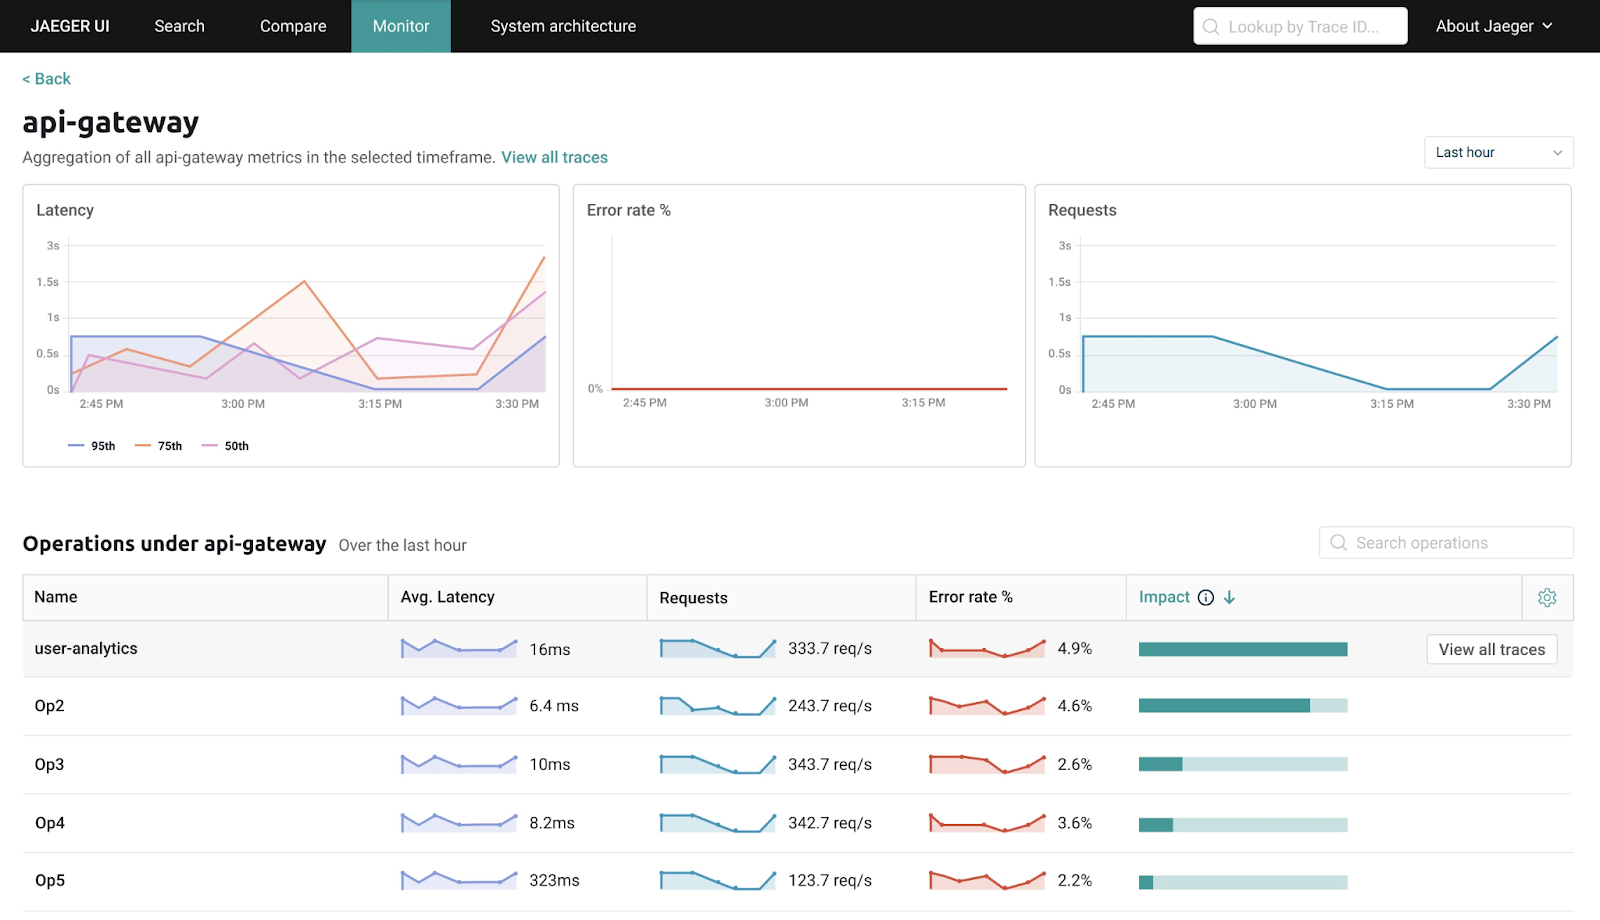
\includegraphics[width=0.98\textwidth]{img/jaeger.png}
                \label{fig:sub1}
                \subcaption{Jaeger interface \cite{otel-p}.}
            \end{subfigure}%
            \begin{subfigure}{.5\textwidth}
                \centering
                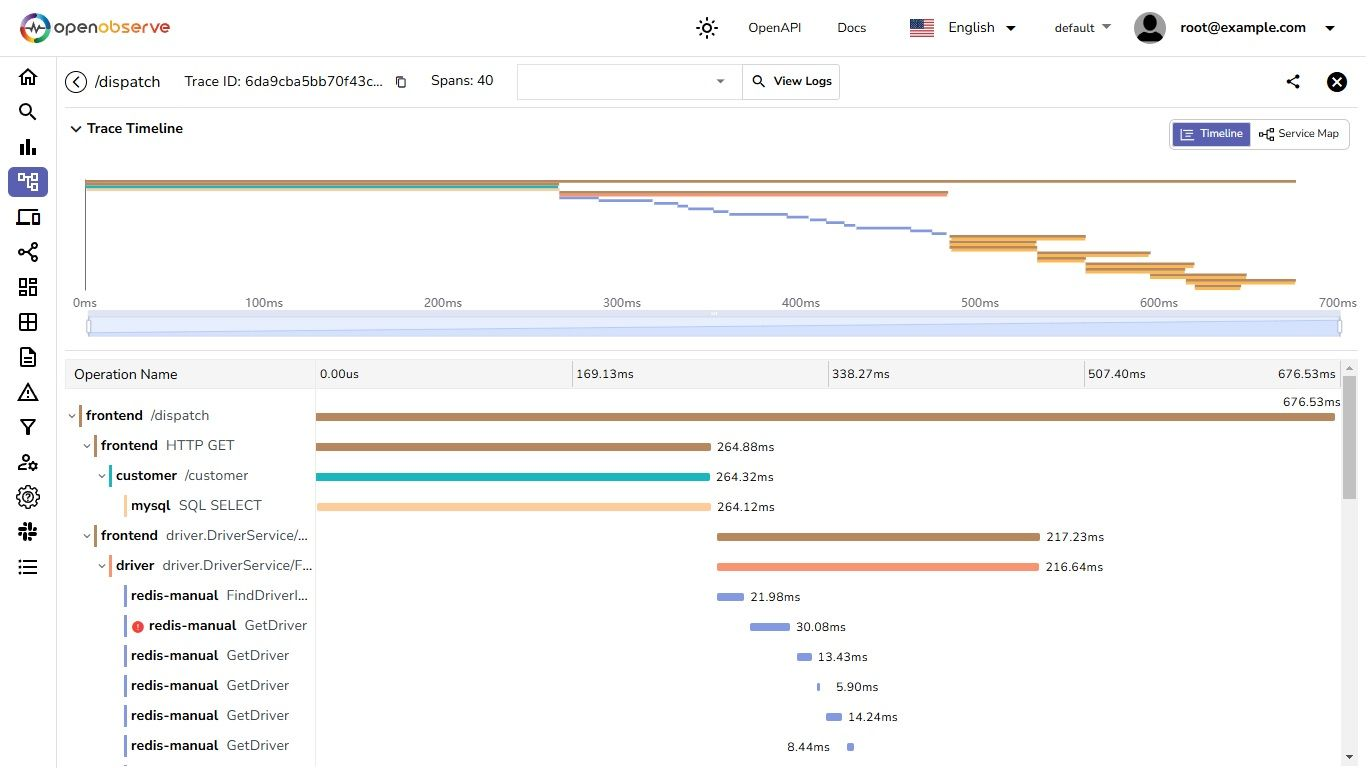
\includegraphics[width =0.98\textwidth]{img/jaeger2.jpg}
                \label{fig:sub2}
                \subcaption{A span analysis on OpenObserve \cite{tr-e} }
            \end{subfigure}
            \label{fig:test}
            \end{figure}


    \subsubsection{Macros}
        OpenTelemetry provides macros to start, end and interact with spans in Erlang, the following code excerpts are taken from the instrumentation wiki. \cite{otel-in}
        \paragraph{?with\_span}
            \texttt{?with\_span} creates active spans. An active span is the span that is currently set in the execution context and is considered the "current" span for the ongoing operation or thread. \cite{active-s}
        \begin{minted}{erlang}
parent_function() ->
    ?with_span(parent, #{}, fun child_function/0).

child_function() ->
    %% this is the same process, so the span parent set as the active
    %% span in the with_span call above will be the active span in this function
    ?with_span(child, #{},
               fun() ->
                   %% do work here. when this function returns, child will complete.
               end).
        \end{minted}

        \paragraph{?start\_span}
            \texttt{?start\_span} creates a span which isn't connected to a particular process, it does not set the span as the current active span.
        \begin{minted}{erlang}
SpanCtx = ?start_span(child),
Ctx = otel_ctx:get_current(),
proc_lib:spawn_link(fun() ->
                        otel_ctx:attach(Ctx),
                        ?set_current_span(SpanCtx),
                        %% do work here
                        ?end_span(SpanCtx)
                    end),
        \end{minted}

        \paragraph{?end\_span}
            \texttt{?end\_span} ends a span started with \texttt{?start\_span}

